
Three variations of the ``CL'' network were made.
The ``CML'' network simply adds a max pooling layer to the convolutional layer.

The ``CLL'' network increases the output units of the convolutional layer and adds a LSTM layer with 64 output units before the final LSTM layer with 3 outputs. This change gives more parameters to the LSTM part of the network.

The ``CLD'' network also tries to increase the influence of the LSTM layer in the network. It reduces the convolutional input window while increases the number of output units. The number of output units of the LSTM network is increased to 128 and a fully connected layer is used as output layer.

The results of the experiments with these variations is shown in table \ref{tab:carvingclvariations}.
Overall, the ``CL'' network and this three variations produced similar results, as can be seen in figure \ref{fig:cl-variations}.

\begin{table}[!ht]
    \centering
    \caption{CL variations}
    \label{tab:carvingclvariations}
\begin{tabular}{r|r|r|r|r|r|r}
\hline
Name & Parameters & Blocks & Epochs & Time    & Training          & Validation          \\       
     &            &        &        &         &          accuracy &            accuracy \\ \hline\hline

CL	    & 24663	    & all	& 150	& 9m29s	    & 0.798	& 0.756 \\hline
CLL	    & 287824	& all	& 108	& 10m00s	& 0.839	& 0.83 \\hline
CML	    & 262416	& all	& 138	& 10m04s	& 0.839	& 0.825 \\hline
CLD	    & 1246339	& all	& 85	& 10m01s	& 0.865	& 0.887 \\hline
\end{tabular}
\end{table}

\begin{figure}[htb!]
\centering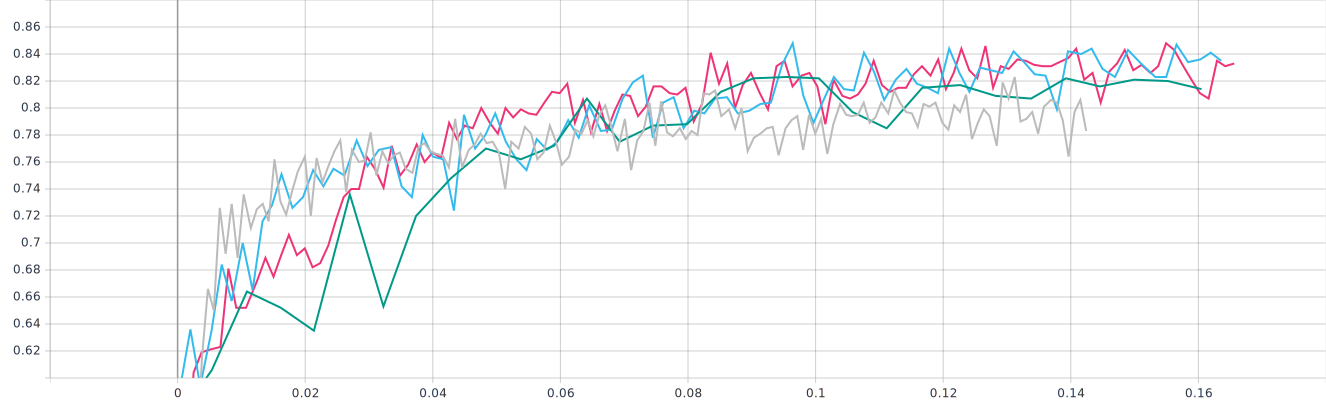
\includegraphics[width=0.65\textwidth]{content/cl-variations.png}
\caption{\label{fig:cl-variations}CL variations}%
\end{figure}
\todo[inline]{legenda}
